\documentclass[tikz,border=0pt]{standalone}
\usepackage[T1]{fontenc}
\usepackage{helvet}
\renewcommand{\familydefault}{\sfdefault}
\usetikzlibrary{arrows.meta,calc}
\tikzset{
 flow/.style={-{Stealth[length=1.7mm,width=1.1mm]},line width=.5pt},
 pics/truck/.style={code={
   % Identical orthographic tractor/trailer geometry for all powertrains.
   \draw (0,2)--(0,7)--(2.5,10)--(7,10)--(7,2)--cycle;
   \draw (1.1,7.2)--(3,9.1)--(5.8,9.1)--(5.8,7.2)--cycle;
   \draw (1,5.8)--(2.4,5.8) (6.2,5.6)--(6.2,6.2);
   \draw (8,3.5) rectangle (29,11);
   \draw (7,2)--(29,2) (8,2)--(8,3.5);
   \foreach \x in {3.5,12,24,27}{
     \draw[fill=white] (\x,1.7) circle (1.65);
     \draw (\x,1.7) circle (.65);
   }
 }},
 metric/.style={draw,minimum width=58mm,minimum height=13mm,inner sep=0pt}
}
\begin{document}
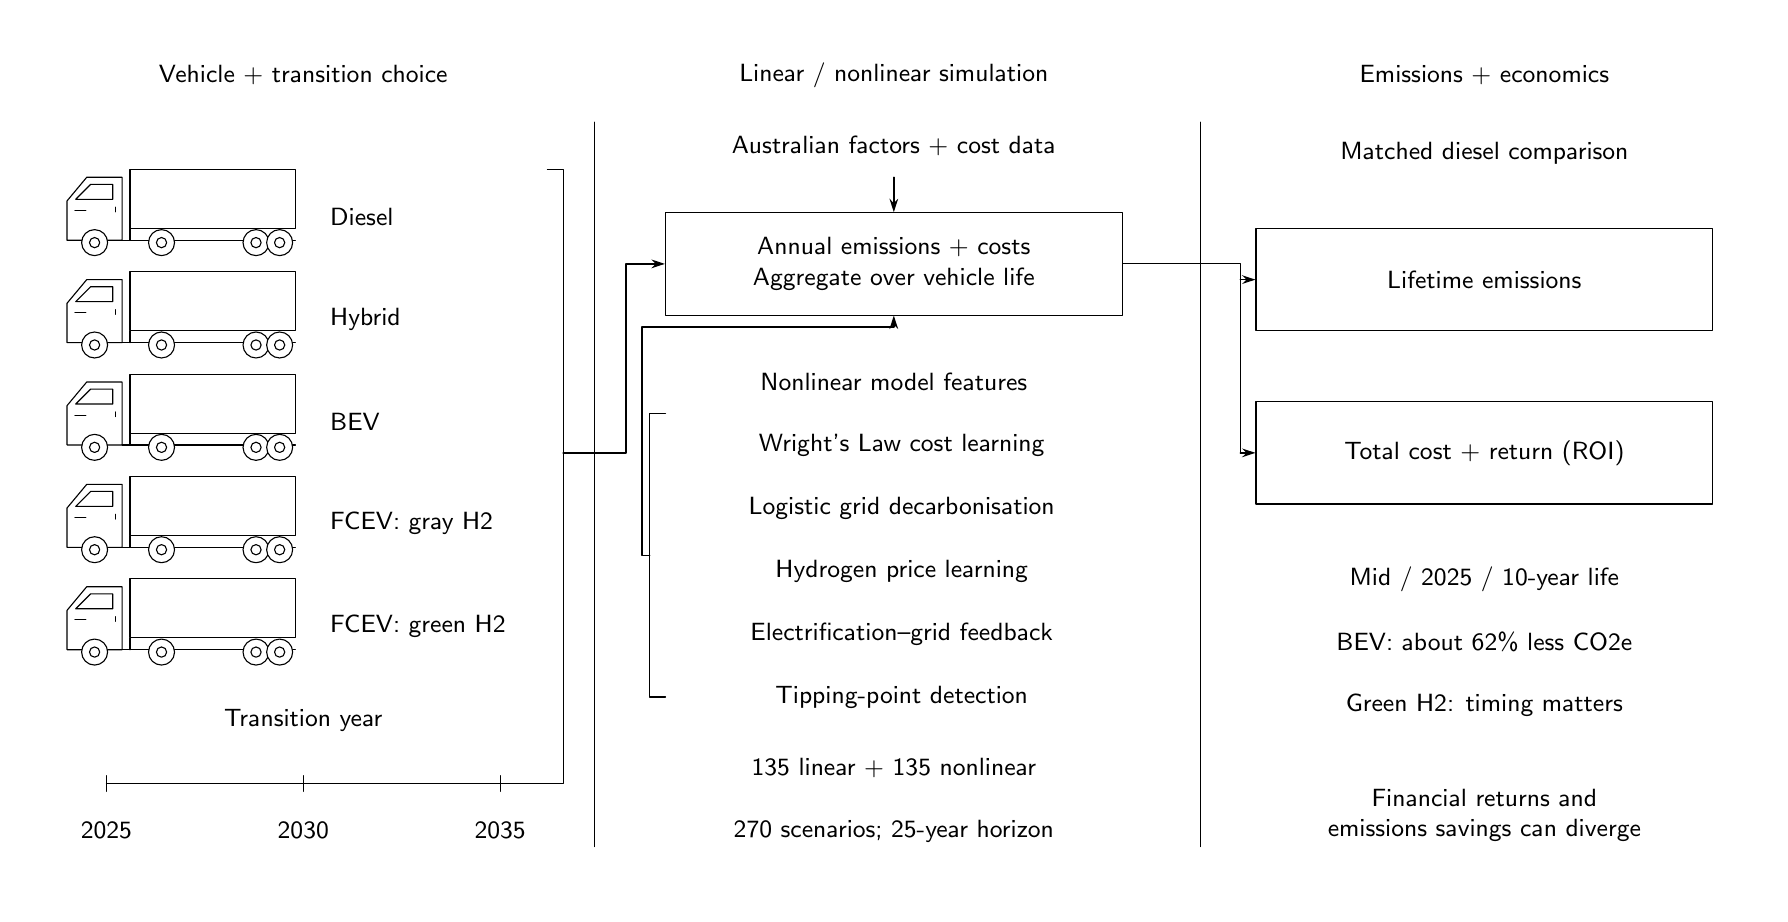
\begin{tikzpicture}[x=1mm,y=1mm,line width=.4pt,line cap=round,line join=round,
 every node/.style={font=\fontsize{9}{11}\selectfont,inner sep=1pt}]
\path[use as bounding box] (0,0) rectangle (220,110);
\node at (35,104) {Vehicle + transition choice};
\node at (110,104) {Linear / nonlinear simulation};
\node at (185,104) {Emissions + economics};
\draw (72,98)--(72,6) (149,98)--(149,6);

% Five choices from the published scenario grid; no hardware detail is asserted.
\foreach \y/\label in {81/Diesel,68/Hybrid,55/BEV,42/FCEV: gray H2,29/FCEV: green H2}{
 \pic at (5,\y) {truck};
 \node[anchor=west] at (38,\y+5) {\label};
}
\node at (35,22) {Transition year};
\draw (10,14)--(60,14);
\foreach \x/\year in {10/2025,35/2030,60/2035}{
 \draw (\x,13)--(\x,15);
 \node at (\x,8) {\year};
}

% Sources feed annual accounting. Mechanisms are shown as model features,
% not as separate observational data streams or five serial computations.
\node at (110,95) {Australian factors + cost data};
\node[metric,align=center] (annual) at (110,80)
 {Annual emissions + costs\\Aggregate over vehicle life};
\draw[flow] (110,91)--(annual.north);
\coordinate (choices) at (68,56);
\draw (66,92)--(68,92)--(68,14)--(60,14);
\draw[flow] (choices)--(76,56)--(76,80)--(annual.west);
\node at (110,65) {Nonlinear model features};
\draw (81,61)--(79,61)--(79,25)--(81,25);
\node at (111,57) {Wright's Law cost learning};
\node at (111,49) {Logistic grid decarbonisation};
\node at (111,41) {Hydrogen price learning};
\node at (111,33) {Electrification--grid feedback};
\node at (111,25) {Tipping-point detection};
\draw[flow] (79,43)--(78,43)--(78,72)--(110,72)--(annual.south);
\node at (110,16) {135 linear + 135 nonlinear};
\node at (110,8) {270 scenarios; 25-year horizon};

% Matched comparison, with no invented curves, points or measured fleet data.
\node at (185,94) {Matched diesel comparison};
\node[metric] (emissions) at (185,78) {Lifetime emissions};
\node[metric] (economics) at (185,56) {Total cost + return (ROI)};
\coordinate (fork) at (154,80);
\draw (annual.east)--(fork)--(154,56);
\draw[flow] (154,78)--(emissions.west);
\draw[flow] (154,56)--(economics.west);
\node at (185,40) {Mid / 2025 / 10-year life};
\node at (185,32) {BEV: about 62\% less CO2e};
\node at (185,24) {Green H2: timing matters};
\node[align=center] at (185,10) {Financial returns and\\emissions savings can diverge};
\end{tikzpicture}
\end{document}
